
\section{Información sobre el proyecto}

\subsection{Sector(es)  en el que se desarrolla el proyecto:}


\subsection{Título:                                        }
\begin{instrucciones}
  El sector puede ser alguno de los propuestos en la convocatoria
  (agricultura, energía, agua, biodiversidad, desarrollo tecnológico e
  innovación) u otros.
\end{instrucciones}
Ciencias Básicas
\subsection{Resumen ejecutivo:                            }
%Máximo 200 palabras.
\subsection{Monto económico total (incluida contrapartida):}
\subsection{Antecedentes:                                  }
Los avances recientes en física de partículas y cosmología han dado
lugar a un entendimiento claro de las tres fronteras a lo largo de la
cual la física de partículas debe avanzar para resolver algunos de los
misterios cruciales de nuestro universo: tales como el origen de la
masa, la naturaleza de la materia oscura y la energía oscura, la
generación de la asimetría materia-antimateria, y la posible
unificación de las fuerzas. Las tres fronteras que se ilustran en la
Figura~\ref{fig:1}, se han identificado como la Frontera de Energía,
la Frontera de Intensidad, y la Frontera Cósmica \cite{fermilab}. Este
proyecto cubrirá las tres frentes y conectará física de partículas y
cosmología. En el proyecto se estudiarán varios modelos teóricos
confrontándolos con los resultados experimentales recientes y haciendo
predicciones para los experimentos en marcha y los que entrarán
próximamente en funcionamiento.

\begin{figure}
  \centering
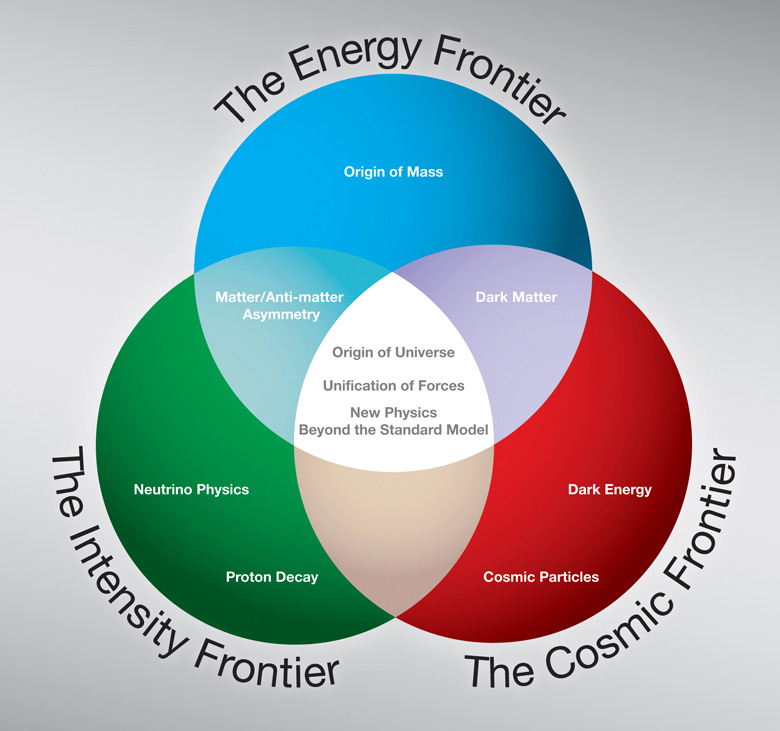
\includegraphics[scale=0.3]{three-frontiers-large}
  \caption{Fronteras de energía. From \cite{fermilab}}
  \label{fig:1}
\end{figure}

Nos encontramos ahora en una época de efervescencia experimental con
detectores de partículas instalados desde las alturas de satélites
artificiales, hasta las profundidades de laboratorios subterráneos a
kilómetros de profundidad. Esto marca una época excitante para la
física de partículas con nuevos datos experimentales disponibles en
las tres fronteras antes mencionadas. La posible correlación de datos
experimentales entre varias de las fronteras podrían permitir un
entendimiento más profundo de los constituyentes del Universo.

La \emph{Frontera de Energía}, ha alcanzado la escala del Tera, la
energía a la cual se rompe la simetría electrodébil con la puesta en
funcionamiento del Large Hadron Collider (LHC). Ubicado en un túnel a
100 metros de profundidad y con una circunferencia de 27 Km, el LHC
posee cuatro detectores, dos de los cuales: ATLAS y CMS, están
especialmente diseñados para encontrar señales de nueva física. El LHC
ha comenzado a operar en el 2010, aunque hasta el 2012 lo hará a la
mitad de la energía para la cual fue diseñado. A partir del 2014
aproximadamente, comenzará a funcionar a la energía de diseño de
14~TeV. Para finales del 2012 el LHC habrá completado su primera fase
de operación a una energía de centro de masa de 7~TeV y habrá
acumulado al menos 8/fb de datos. Con esta luminosidad se podrá
vislumbrar una escala de energía que hasta ahora no había sido
explorada. La prioridad es la búsqueda del Higgs del Modelo Estándar,
el cual a la fecha aún no ha sido encontrado. Pero para comienzos del
2011 se espera obtener la primeras evidencias de su existencia o
excluirlo hasta un rango de masa de unos 600~GeV.

Quizás el resultado experimental más importante en los últimos años de
necesidad de física más allá del modelo estándar (ME) de las
partículas elementales es el descubrimiento de que los neutrinos
tienen masa, las cuales han resultado ser pequeñas aunque diferentes de
cero. Las diferencias de masa al cuadrado de neutrinos, además de sus
correspondientes ángulos de mezcla, son necesarios para poder explicar
las observaciones de oscilaciones de neutrinos a medida que se
propagan sobre grandes distancias. Debido a que los neutrinos
interactúan sólo débilmente, los experimentos de neutrinos requieren
de detectores fabricados de materiales masivos y rayos muy
intensos. Los experimentos de neutrinos exploran de ésta manera la
\emph{Frontera de Intensidad}. Los experimentos en esta frontera se
enfocan ahora en estudios más precisos de oscilaciones de neutrinos
así como en búsqueda de nuevas fuentes de violación de CP, mezcla de
sabores de leptones cargados, decaimientos raros, y en la
determinación de la velocidad de propagación de neutrinos
energéticos. Los experimentos que usan rayos muy intensos a energías
inferiores que el LHC pueden proveer información complementaria a los
posibles descubrimientos de los detectores ATLAS y CMS. Un decaimiento
raro que proviene del intercambio de una partícula de masa alta puede
contener información sobre las propiedades del estado intercambiado
aunque éste sea demasiado pesado para ser producido directamente.

Recientemente se ha venido acumulando evidencia experimental respecto
al ángulo de mezcla del sector de neutrinos que aún falta por
determinar, mostrando que dicho ángulo no sólo es diferente de cero
sino que puede ser suficientemente grande como para permitir violación
de CP en el sector leptónico \cite{valle}. La violación de CP en el
sector leptónico es un ingrediente necesario para generar la asimetría
de materia-antimateria a través de
leptogénesis~\cite{Davidson:2008bu}.


La \emph{Frontera Cósmica} utiliza laboratorios subterráneos,
telescopios basados en tierra y telescopios instalados en satélites
para explorar la componentes oscuras de materia y energía, las huellas
de la inflación y el origen y destino del universo. Las observaciones
de la Frontera Cósmica han alcanzado una precisión mucho mayor de la
podría haber sido imaginada dos décadas antes. Estos han conseguido
determinar detalles del universo primitivo los cuales son cada vez más
consistentes con el ``Modelo Estándar'' de Cosmología basado en la
constante cosmológica y en la materia oscura fría ($\Lambda$CDM), que
dan cuenta del 95\% del contenido energético del Universo. Técnicas
novedosas como lentes gravitacionales, han aportado significativamente
a nuestro conocimiento del pasado cosmológico, en particular en
aumentar la evidencia experimental de que la materia oscura del
universo está compuesta de partículas masivas débilmente
interactuantes (WIMPS), formando halos de materia alrededor de las
galaxias. Cómo los neutrinos constituyen sólo alrededor del 0.5\% del
contenido energético del universo, los WIMPS deben corresponder a
nuevas partículas no presentes en el ME, constituyéndose en la segunda
evidencia experimental de necesidad de física más allá del ME. Estas
partículas deben ser o bien estables, o inestables pero con un tiempo
de vida mayor que la edad del universo, generando productos de
aniquilación en el primer caso, o de decaimiento en el segundo
generando rayos cósmicos que pueden llegar a los detectores instalados
en satélites artificiales orbitando la tierra.  El valor de múltiples
estudios con detectores de diversos tipos de partículas y radiación
electromagnética sobre un rango muy amplio (incluyendo rayos gamma) se
hace evidente en el conocimiento detallado que se ha logrado alcanzar
y el que se espera mejorar con los experimentos que recientemente han
entrado en funcionamiento.

Desde el 2008 varios experimentos sobre rayos cósmicos como ATIC
\cite{:2008zzr} y los satélites PAMELA \cite{Adriani:2008zr} y
Fermi--LAT \cite{Abdo:2009zk}, han venido reportando un exceso en el
flujo de electrones y positrones en rayos cósmicos. Estos resultados
han dado lugar a un sinnúmero de publicaciones tratando de explicar su
origen. Las medidas cada vez más precisas de rayos gamma por parte de
Fermi--LAT, pueden ayudar a discernir si el origen de las anomalías
detectadas en electrones y positrones es debida a fuentes astrofísicas
como pulsares cercanos, o a la aniquilación o el decaimiento de
materia oscura. El detector de rayos cósmicos AMS-02~\cite{ams:2009},
ha sido instalado recientemente en la estación espacial internacional
para medir el espectro de antiprotones y positrones en un rango de
energía mucho más amplio y con una estadística mucho mejor que PAMELA.

Los experimentos de detección directa de materia oscura instalados en
laboratorios subterráneos como XENON100 \cite{Aprile:2011ts}, han
comenzado a explorar las regiones predichas por algunos de los modelos
más estudiados de materia oscura. Para los próximos años se espera
cubrir todo el espacio de parámetros para materia oscura del modelo
estándar supersimétrico mínimo restringido (Constrained MSSM de sus
siglas en Inglés).  

\subsection{Justificación:                                 }
\begin{instrucciones}
  CODI: 

  * ¿Está bien definido el problema que se quiere investigar?:
  Fenomenología de modelos más allá del ME motivados por evidencias
  fenomenológicas del ME.  
  * ¿Es clara su justificación desde el punto de vista académico,
  científico, tecnológico, social, económico y legal? (15).
  científico: contribuir a la correspondiente rama del conocimiento

  COLCI: en este ítem usted deberá describir de forma precisa y completa la
  
  * naturaleza y magnitud del problema de investigación que se quiere
  abordar:
  ** Construir modelos nuevos.
  ** Explorar modelos existentes.
  Formule claramente las preguntas concretas a las cuales se
  quiere responder en el contexto del problema planteado.
\end{instrucciones}
%Tesis
El Grupo de Fenomenología de Interacciones Fundamentales de la
Universidad de Antioquia, en colaboración con Grupos emergentes en
otras instituciones la región conformados por egresados de doctorado
de nuestro Grupo, se ha enfocado en la investigación científica de
aspectos fenomenológicos en estas tres fronteras de la física de altas
energías y la cosmología. Estas investigaciones se han hecho en
colaboración con investigadores internacionales, especialmente con
científicos colombianos trabajando en el exterior. A través de este
proyecto se busca dar continuidad a estos desarrollos a través de
investigaciones de impacto científico en la comunidad científica de
éstas áreas de frontera. En éste proyecto se explorarán diferentes
extensiones del modelo estándar que explican estos datos y tienen
predicciones concretas para los experimentos presentes y futuros en
éstas tres fronteras de la física de partículas y la cosmología.

Si la masa de los neutrinos es total o parcialmente explicada por
métodos radiativos, no sólo es posible dar cuenta de la pequeñez de
sus masas con respecto a la de los otros fermiones, sino también,
hacer predicciones muy concretas en aceleradores de partículas, como
el LHC. 


  %evidencia 4
Las observaciones astronómicas sugieren que el Universo está compuesto
en su mayor parte de materia. En el contexto del big-bang, esto
implica que en algún momento grandes cantidades de materia y
antimateria se aniquilaron dejando el pequeño exceso de materia que
constituye el Universo observable actual. El problema de explicar el
exceso inicial de materia sobre antimateria se conoce con el nombre de
bariogénesis. Dentro del modelo estándar, aunque contiene los
ingredientes necesarios, no es posible explicar bariogénesis.

%conclusion
Un modelo ideal sería uno que de cuenta de las masas y mezclas de
neutrinos, tenga un candidato a materia oscura que sirva para explicar
el exceso de positrones en experimentos de rayos cósmicos y a la vez
contenga los ingredientes para explicar bariogénesis.  En este
proyecto pretendemos formular un modelo de éstas características,
además queremos continuar explorando otros posibles modelos que puedan
dar cuenta de alguna de las evidencias fenomenológicas (masas de
neutrinos o materia oscura) que requieren una extensión del modelo
estándar.


\begin{proyecto}
  Con base en lo planteado anteriormente, lo que proponemos en este
  proyecto es tratar de responder la siguiente pregunta: ¿Cuáles
  serían las restricciones impuestas por los resultados experimentales
  presentes y futuros de los experimentos de física de partículas
  sobre modelos que presenten una partícula candidata a materia oscura
  o que generen masas para los neutrinos?
\end{proyecto}
 

\subsection{Objetivos:                                     }
\subsection{Metodología:                                   }
\subsection{Actividades:                                   }
\subsection{Resultados esperados:                          }
\subsection{Cronograma:                                    }

\subsection{Equipo de trabajo:}
\begin{tabular}{|l|l|l|l|}\hline
Recurso humano (rol)& Responsabilidad& Unidades (días, meses)& \# de unidades\\\hline
&&&\\\hline
\end{tabular}

\subsection{Presupuesto}
\begin{instrucciones}
  Por favor siga el modelo de la tabla que encontrará en este punto para la presentación del presupuesto.
\end{instrucciones}
\begin{tabular}{|l|l|l|l|}\hline
  \multirow{2}{*}{Rubros}&\multicolumn{2}{c}{Fuentes}\vline&\multirow{2}{*}{Total}\\
  \cline{2-3} & Colciencias & Contrapartida & \\\hline 
 & & &\\\hline
 & & &\\\hline
 & & &\\\hline
 & & &\\\hline
TOTAL (en pesos) & & &\\\hline
Total en porcentaje & & &\\\hline
\end{tabular}

\subsection{Plan de acción.}
\begin{tabular}{|l|l|l|l|l|l|}\hline
  \multirow{2}{*}{Objetivo} & \multirow{2}{*}{Estrategia} & \multirow{2}{*}{Indicador}  & \multicolumn{3}{|c|}{Metas}\\
\cline{4-6} 
& & & Bimestre 1 &Bimestre 2 & Bimestre 3\\\hline 
&&&&&\\\hline
\end{tabular}



%%% Local Variables: 
%%% mode: latex
%%% TeX-master: "proyecto"
%%% End: 
